\documentclass[a4paper,english]{report}
\usepackage[utf8]{inputenc}
\usepackage{babel}
\usepackage[backend=biber]{biblatex}
\bibliography{library.bib}
\usepackage{csquotes}
\usepackage{pdfpages}
\usepackage{graphicx}
\usepackage{mathtools}
\usepackage{amsmath}
\usepackage{amssymb}
\usepackage{subcaption}

\usepackage{titlesec}
\begin{document}

\section{PathNet}\label{pathnet}
In 2017 DeepMind took the modular approach\footnote{Modular with respect to the traditional approaches of transfer from monolithic models} to deep transfer learning for multi-task systems one step further with their newly developed PathNet. Where PNNs transfer knowledge between domains by adding new uninitialized DNNs for each task, the size of PathNet is not dynamic in the number of parameters. At training start, the net consist of randomly initialized weights in multiple DNNs, where each DNN is considered a module (or node) in a larger network of DNNs. 

Using a combination of evolutionary and machine learning techniques, PathNet share the PNNs traits of being able to optimize for multiple training tasks without catastrophic forgetting, and transfer knowledge between tasks by reusing locked weights.  

For each training task, a set of pathways through the network are initialized as phenotypes and evaluated through a set duration training period using gradient descent where all parameters along the phenotypes path are updated and it fitness evaluated as a function of the loss through this path. Through a tournament selection algorithm, the variation in the genotype decrease and the set of paths converge on one optimal path through the net for the current task. The weights along this path is then locked to future back propagation, and all other weights are reinitialized randomly.
\begin{figure}[t]
    \label{fig:pathnet}
    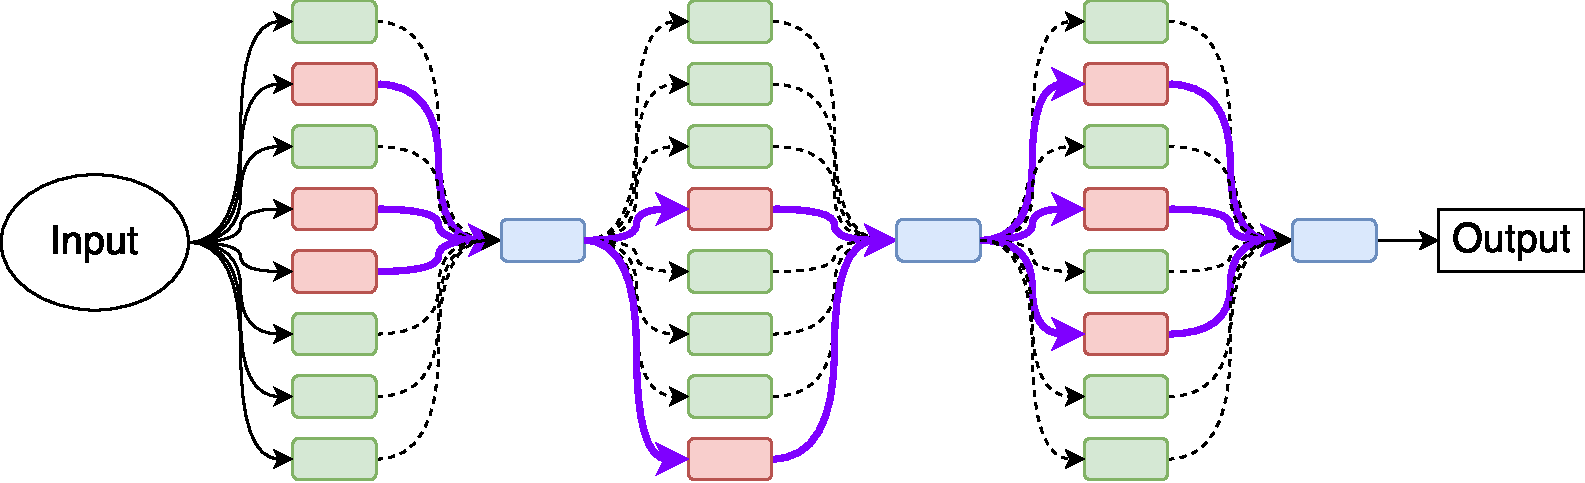
\includegraphics[width=\textwidth]{figures/PathNet.pdf}
    \caption{Figure shows a PathNet implementation with 3 layers of 8 modules (DNNs) in each layer. The \textit{red} color indicates the weights of this DNN is locked from back propagation, while \textit{green} indicates it is open. \textit{Blue} cells are reduced sum modules which summarizes the feature maps between each layer.The purple connections shows a possible optimal path for a task. One path may use multiple modules from each layer.}
\end{figure}
This locking of parameters is the preventive measure that keeps fine tuning of weights from destructively influence previously learned tasks, but is also the limitation to number tasks the net is able to learn. As the number of tasks applied to PathNet increase, the number of locked parameters increase, and at some point, the net is locked from future learning. At that point, new knowledge would have to be encoded in the NN solely as a new path, and the algorithm responsible for this learning would, in the case of DeepMinds implementation, be the tournament search. The paper also states other evolutionary techniques could be applied and even a RL-system, but this is not addressed.

While the process of evolving paths through tournament search alone might be a must for learning new tasks when the NN is fully locked, this might happen for a large net while some modules are still open. As the paper on PNNs showed, the capacity needed for new tasks diminish over number of tasks learned if transfer learning is sufficiently achieved. Might a saturation point in a PathNet be reached, where previously gained knowledge saved in the modules may be used efficiently enough for new knowledge to be based on these modules alone? 

\end{document}